\documentclass{beamer} 
\usepackage[utf8]{inputenc}
\usepackage[T1]{fontenc} 
\usepackage[slovene]{babel} 
\usepackage{lmodern}
\usepackage{amsfonts} 
\usepackage{enumitem} 
\usepackage{mathtools}
\usepackage{amsmath}
\usepackage{amsthm} 

\newcommand{\overbar}[1]{\mkern 1.5mu\overline{\mkern-1.5mu#1\mkern-1.5mu}\mkern 1.5mu}


\usetheme{Warsaw}
\beamertemplatenavigationsymbolsempty
\setbeamertemplate{caption}[numbered]

\title{Schwarzov princip zrcaljenja za harmonične funkcije}
\author{Matej Novoselec}
\institute[UL FMF]{FMF Fakulteta za matematiko in fiziko}
\date{4. september 2023}


\theoremstyle{definition}
\newtheorem{defi}{Definicija}[section]
\theoremstyle{definition}
\newtheorem{op}[defi]{Opomba}
\newtheorem{trditev}{Trditev}
\newtheorem{lema}{Lema}
\newtheorem{izrek}{Izrek}

\begin{document}
%----------------------------------
\begin{frame}
   \titlepage
\end{frame}
%----------------------------------
%---------------------------------
%\begin{frame}{Harmonične funkcije}
%    \begin{block}{Definicija}
%        Naj bo $U$ odprta podmnožica v $\mathbb{R}^n$. Naj bo $u$ funkcija, definirana na $U$ in naj bo na definicijskem območju dvakrat zvezno odvedljiva.  
%        Pravimo, da je funkcija $u(x_1, x_2, \dots, x_n)$ \textbf{harmonična}, če velja
%        $$
%        \frac{\partial^2 u}{\partial x_1 ^ 2} +  \frac{\partial^2 u}{\partial x_2 ^ 2} + \dots + \frac{\partial^2 u}{\partial x_n ^ 2} = 0.
%        $$
%        Operatorju $\Delta  = \frac{\partial^2}{\partial x_1 ^ 2} +  \frac{\partial^2}{\partial x_2 ^ 2} + \dots + \frac{\partial^2}{\partial x_n ^ 2}$ pravimo \textbf{Laplaceov operator} in pišemo
%        $$
%        \Delta u = 0.
%        $$
%    \end{block}
% \end{frame}

%\begin{frame}{Holomorfne funkcije}
%   \begin{alertblock}{Izrek (Cauchyjeva formula)}
%    Naj bo $D$ območje, ki zadošča pogojem za Greenovo formulo. 
%    Naj bo $f \in \mathcal{O}(D) \cap \mathcal{C}^1(\overline{D})$. 
%    Potem za $z \in D$ velja 
%    $$
%    f(z) = \frac{1}{2 \pi i} \int_{\partial D}{\frac{f(\xi)}{\xi - z}~d\xi}.
%    $$
%   \end{alertblock}
%   \pause
%    \begin{alertblock}{Izrek (Princip maksima za holomorfne funkcije)}
%        Naj bo $f$ kompleksna holomorfna funkcija, definirana na območju $D$. 
%        Naj obstaja $M \in \mathbb{R}$, da za vsak $z \in D$ velja $|f(z)| \leq M $. 
%        Če obstaja $z_0 \in D$, da velja $|f(z_0)| = M$, potem je $f$ na $D$ konstantna.  
%   \end{alertblock}
%\end{frame}
%----------------------------------
\begin{frame}{Lastnost povprečne vrednosti}
    \begin{block}{Definicija (Lastnost povprečne vrednosti)}
        Naj bo $h$ kompleksna zvezna funkcija, definirana na območju $D$. Pravimo, da ima funkcija $h$ na $D$ \textbf{lastnost povprečne vrednosti}, če za vsak $z_0 \in D$ obstaja $\epsilon_0 > 0$, da je $\overline{\mathbb{D}}(z_0, \epsilon_0) \subseteq D$ in za vsak $0 < \epsilon \leq \epsilon_0 $ velja
        $$
            h(z_0) = \frac{1}{2 \pi} \int_{0}^{2 \pi}{h(z_0 + \epsilon e^{i \theta}) d\theta}.
        $$
    \end{block}
    \pause
     \begin{alertblock}{Izrek (Princip maksima za funkcije z lastnostjo povprečne vrednosti)}
        Naj bo $h$ zvezna kompleksna funkcija, definirana na območju $D$. Naj ima $h$ na $D$ lastnost povprečne vrednosti in naj obstaja $M \in \mathbb{R}$, da velja $|h(z)| \leq M$ za vsak $z \in D$. 
        Če obstaja $z_0 \in D$, da je $|h(z_0)| = M$, potem je funkcija $h$ na $D$ konstantna. 
    \end{alertblock}
 \end{frame}


\begin{frame}{Dirichletov problem za enotski disk}
    \begin{exampleblock}{Dirichletov problem za enotski disk}
        Naj bo $h$ kompleksna zvezna funkcija, definirana na $\partial \mathbb{D}$. 
        Ali obstaja razširitev $H$, ki je zvezna na $\overbar{\mathbb{D}}$ in harmonična na $\mathbb{D}$?
    \end{exampleblock}
    \begin{figure}
    \begin{center}
      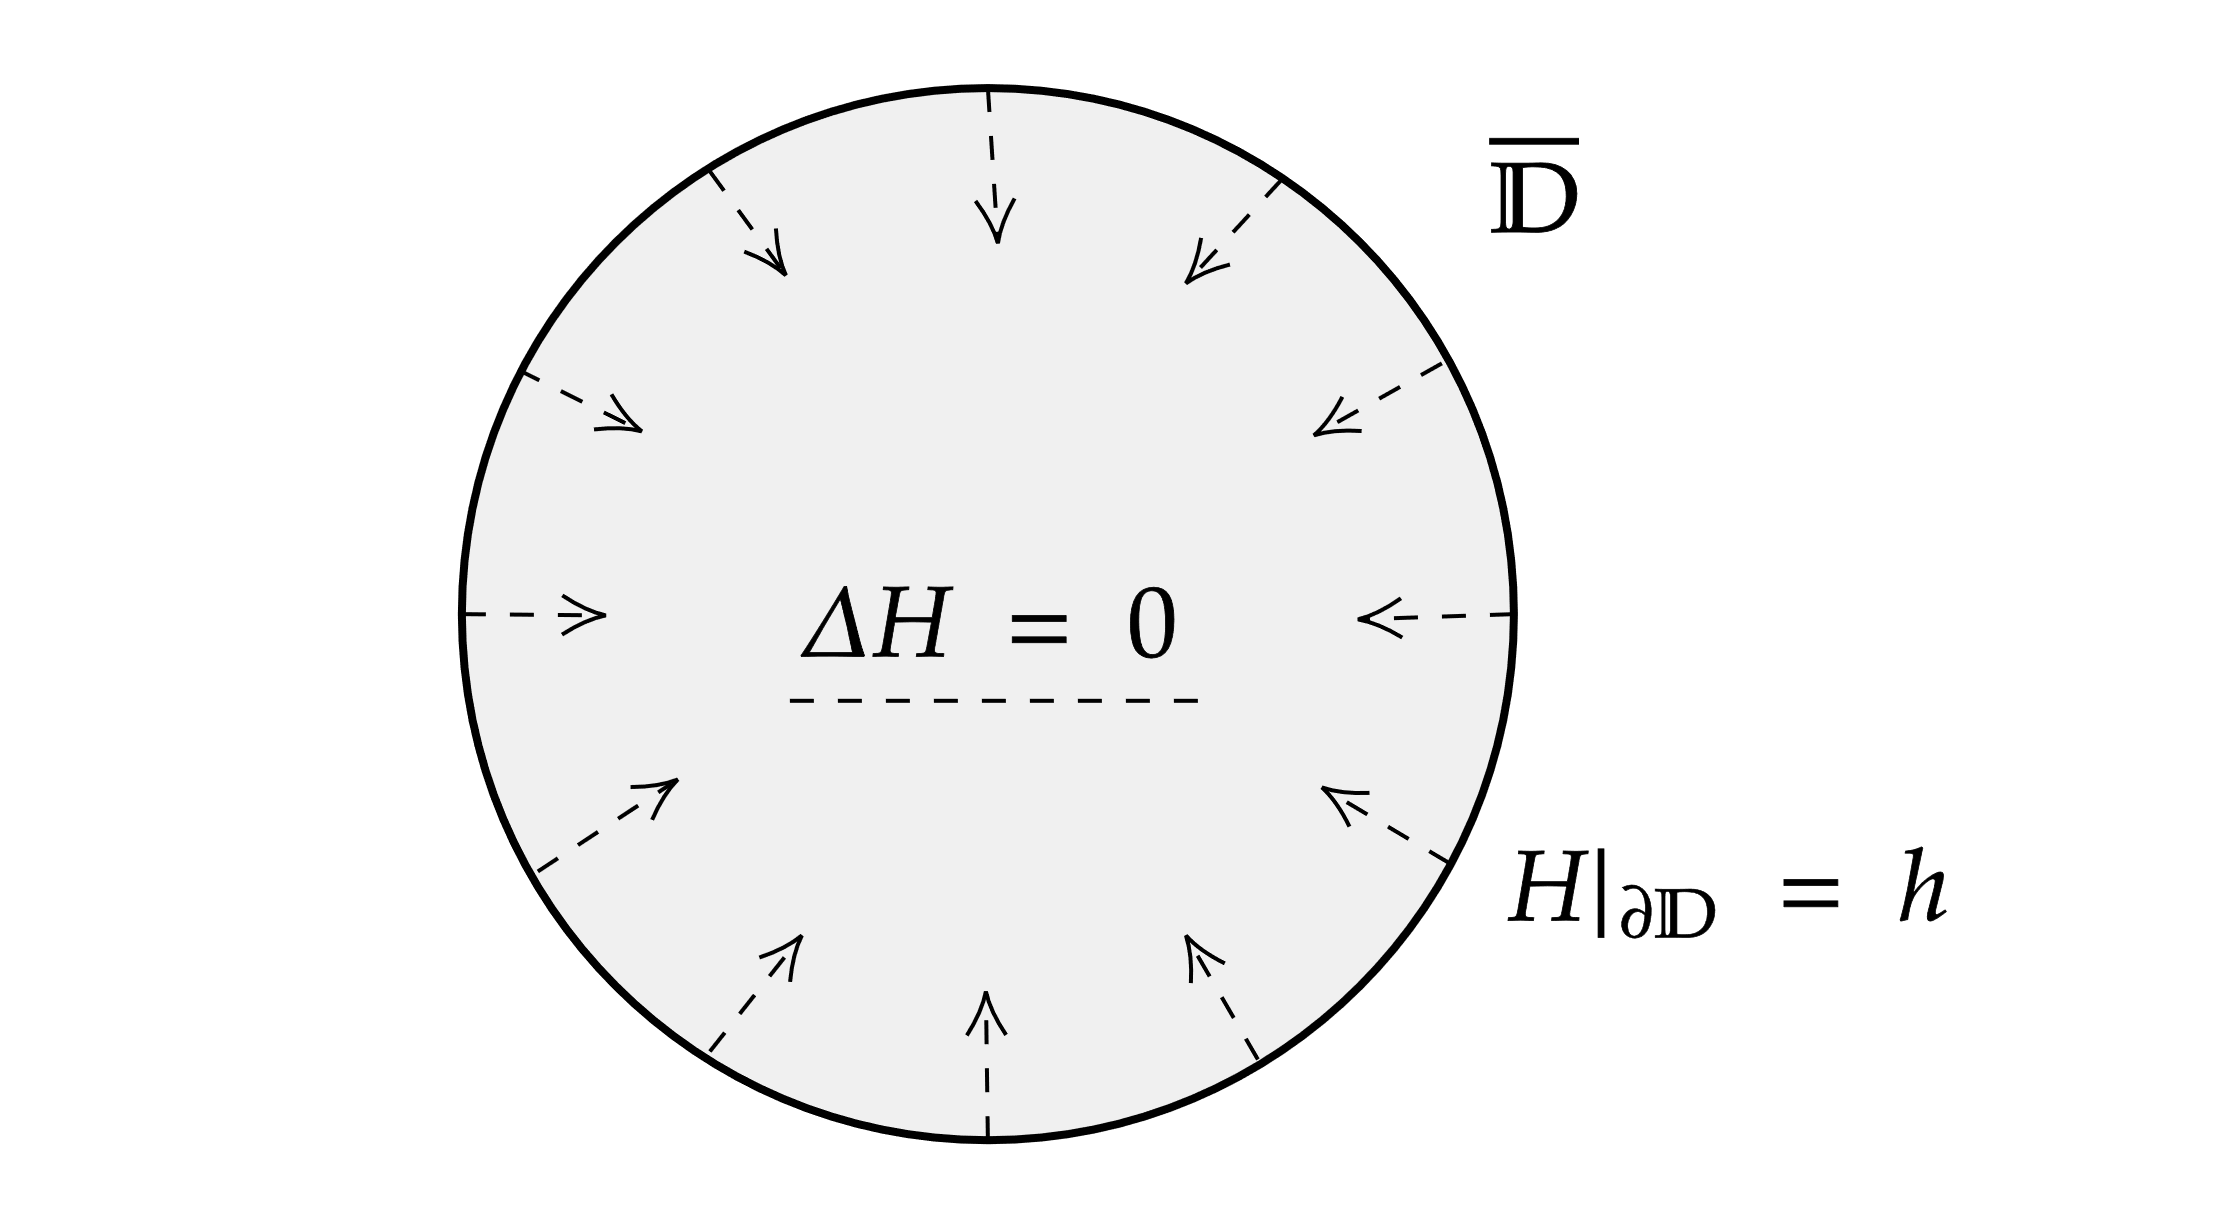
\includegraphics[width=0.8 \textwidth]{dirichlet_form.png}
    \end{center}
    \end{figure}
\end{frame}

\begin{frame}{Reševanje Dirichletovega problema za enotski disk}
    \begin{block}{Definicija}
        \textbf{Poissonovo jedro} je funkcija, definirana s predpisom
        $$
           P_r(\theta) = \sum_{k = -\infty}^{\infty}{r^{|k|} e^{i k \theta}}\text{, kjer je}~\theta \in [-\pi, \pi]~\text{in}~ 0 \leq r < 1.
        $$
    \end{block}
    \pause
    \begin{block}{Definicija}
        Naj bo $h$ zvezna funkcija, definirana na robu enotskega diska.
        \textbf{Poissonov integral} funkcije $h$, ki ga označimo s $\widetilde{h}$, je funkcija, definirana na notranjosti enotskega diska s predpisom
        $$
        \widetilde{h}(z) = \int_{0}^{2\pi}{h(e^{i\varphi}) P_r(\theta - \varphi)~\frac{d\varphi}{2 \pi}}~,~~z = r e^{i\theta} \in \mathbb{D}.
        $$
    \end{block}
\end{frame}

\begin{frame}{Rešitev Dirichletovega problema za enotski disk}
    \begin{alertblock}{Izrek}
        Naj bo $h$ zvezna kompleksna funkcija, definirana na $\partial \mathbb{D}$. Rešitev Dirichletovega problema, z robnim pogojem $h$, za enotski disk obstaja in je na $\mathbb{D}$ definirana kot Poissonov integral funkcije $h$.
    \end{alertblock}
    \begin{figure}
    \begin{center}
      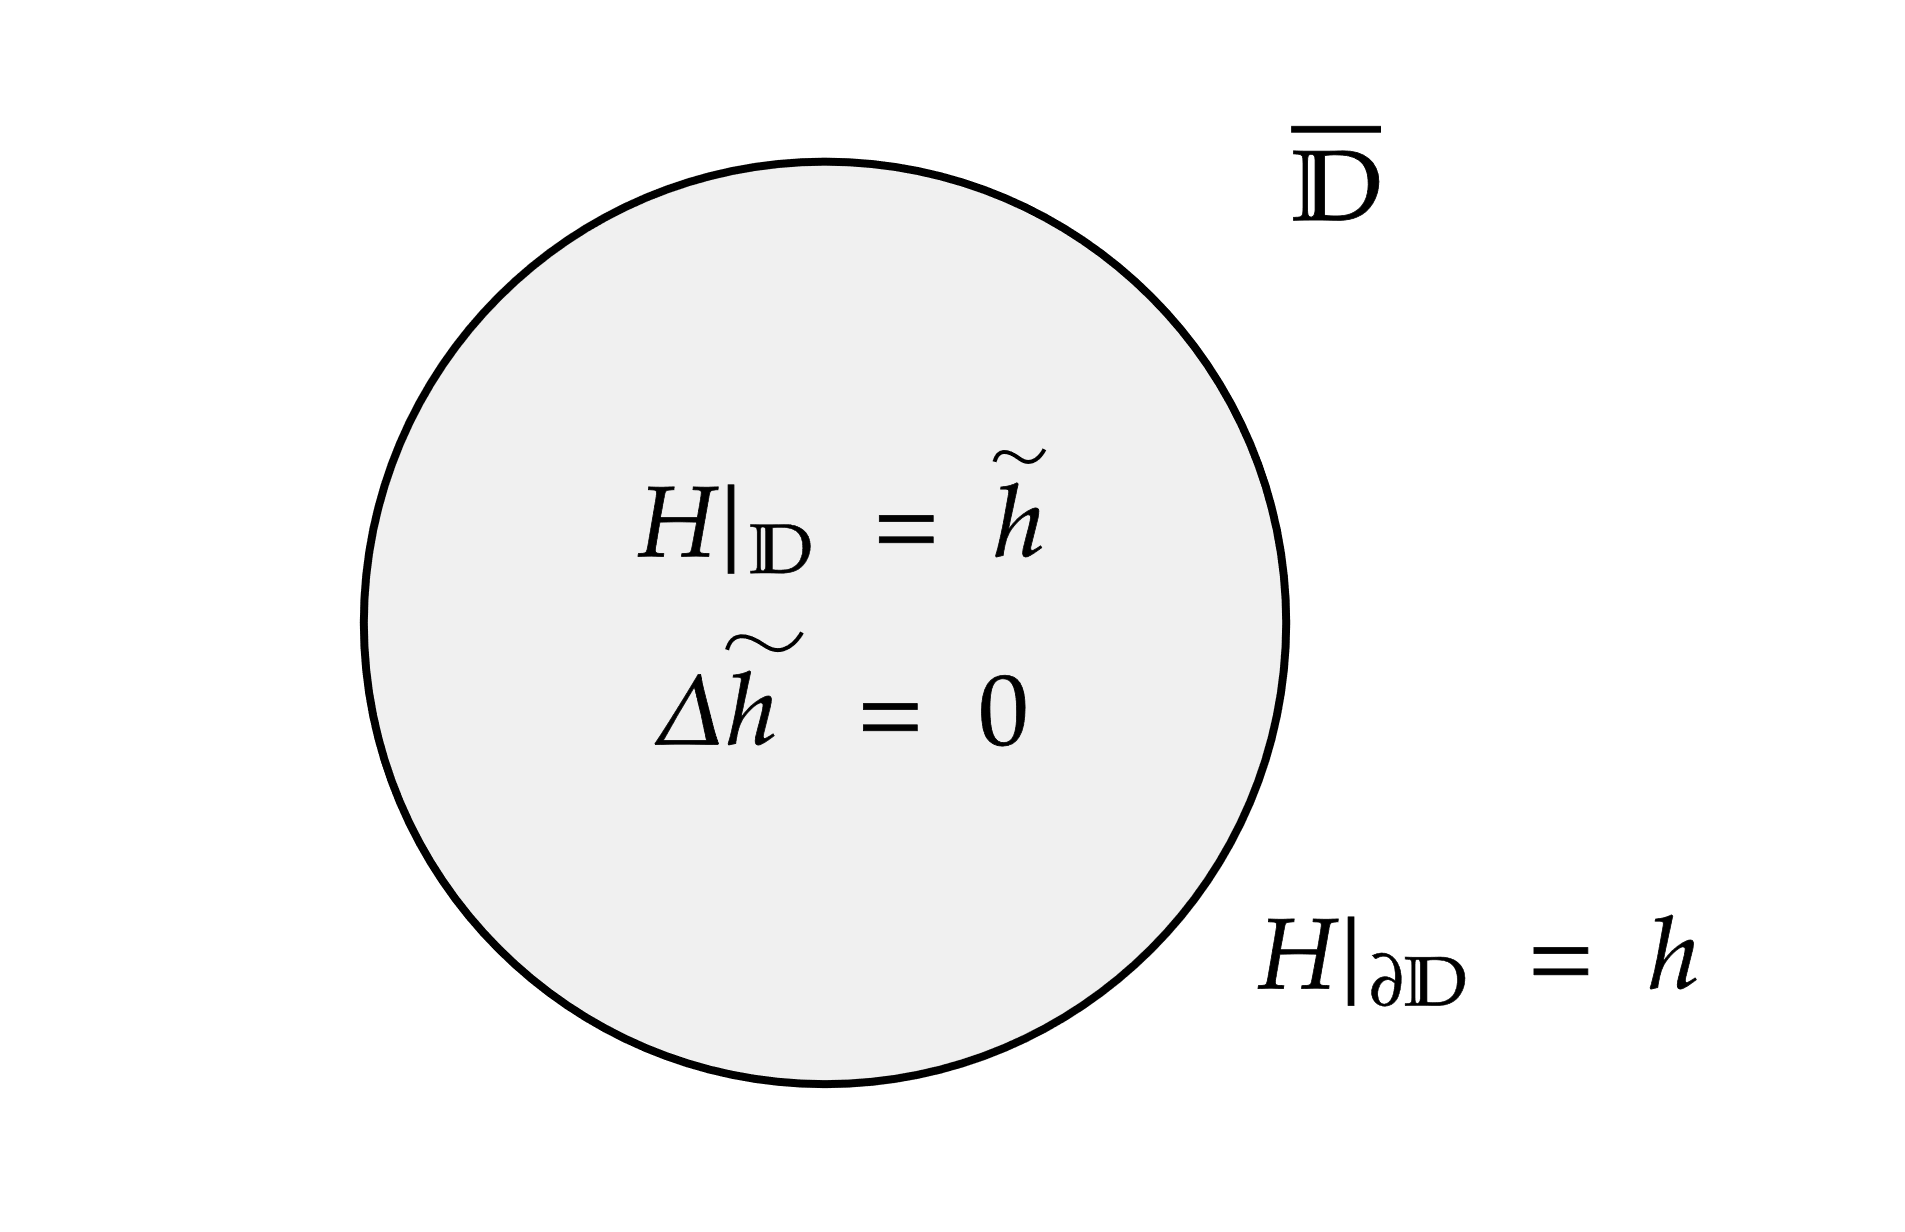
\includegraphics[width=0.8 \textwidth]{dirichlet_resitev.png}
    \end{center}
    \end{figure}
\end{frame}

\begin{frame}{Karakterizacija harmoničnih funkcij}
    \begin{alertblock}{Izrek (Karakterizacija harmoničnih funkcij)}
        Naj bo $h$ zvezna funkcija, definirana na območju $D \subseteq \mathbb{C}$. Velja, da je $h$ harmonična funkcija natanko tedaj, ko ima na $D$ lastnost povprečne vrednosti.
    \end{alertblock}
    \pause
    \begin{alertblock}{Izrek Morera}
        Naj bo $D$ območje in $f$ kompleksna zvezna funkcija, definirana na $D$. 
        Denimo, da za vsak zaprt trikotnik $T \subseteq D$ velja 
        $$
        \int_{\partial T} {f(\xi)~d\xi} = 0.
        $$
        Tedaj je $f$ holomorfna na $D$.
    \end{alertblock}
\end{frame}

\begin{frame}{Schwarzov princip zrcaljenja za harmonične funkcije}
    \begin{exampleblock}{Izrek (Schwarzov princip zrcaljenja za harmonične funckije)}
        Naj bo $D \subseteq \mathbb{C}$ območje, simetrično glede na realno os. 
        Označimo $D^{+} = \{z \in D~|~\text{Im}[z] > 0\},~D^{-} = \{z \in D~|~\text{Im}[z] < 0\}$ in $D^{0} = \{z \in D~|~\text{Im}[z] = 0\}$.
        Naj bo $u$ realna zvezna funkcija, definirana na $D^{+} \cup D^0$. Naj bo $u$ na $D^{+}$ harmonična in naj za vsak $z \in D^0$ velja $u(z) = 0$.
        Potem je funkcija $U$, definirana s predpisom
        $$
        U(z) = 
        \begin{cases}
            u(z)~~~,~~z \in D^{+}\\
            ~0~~~~~~,~~z \in D^0\\
            -u(\overbar{z})~,~~z \in D^{-}
        \end{cases},
        $$
        na območju $D$ harmonična.
    \end{exampleblock}
\end{frame}

\begin{frame}{Schwarzov princip zrcaljenja za harmonične funkcije}
   \begin{figure}
   \begin{center}
      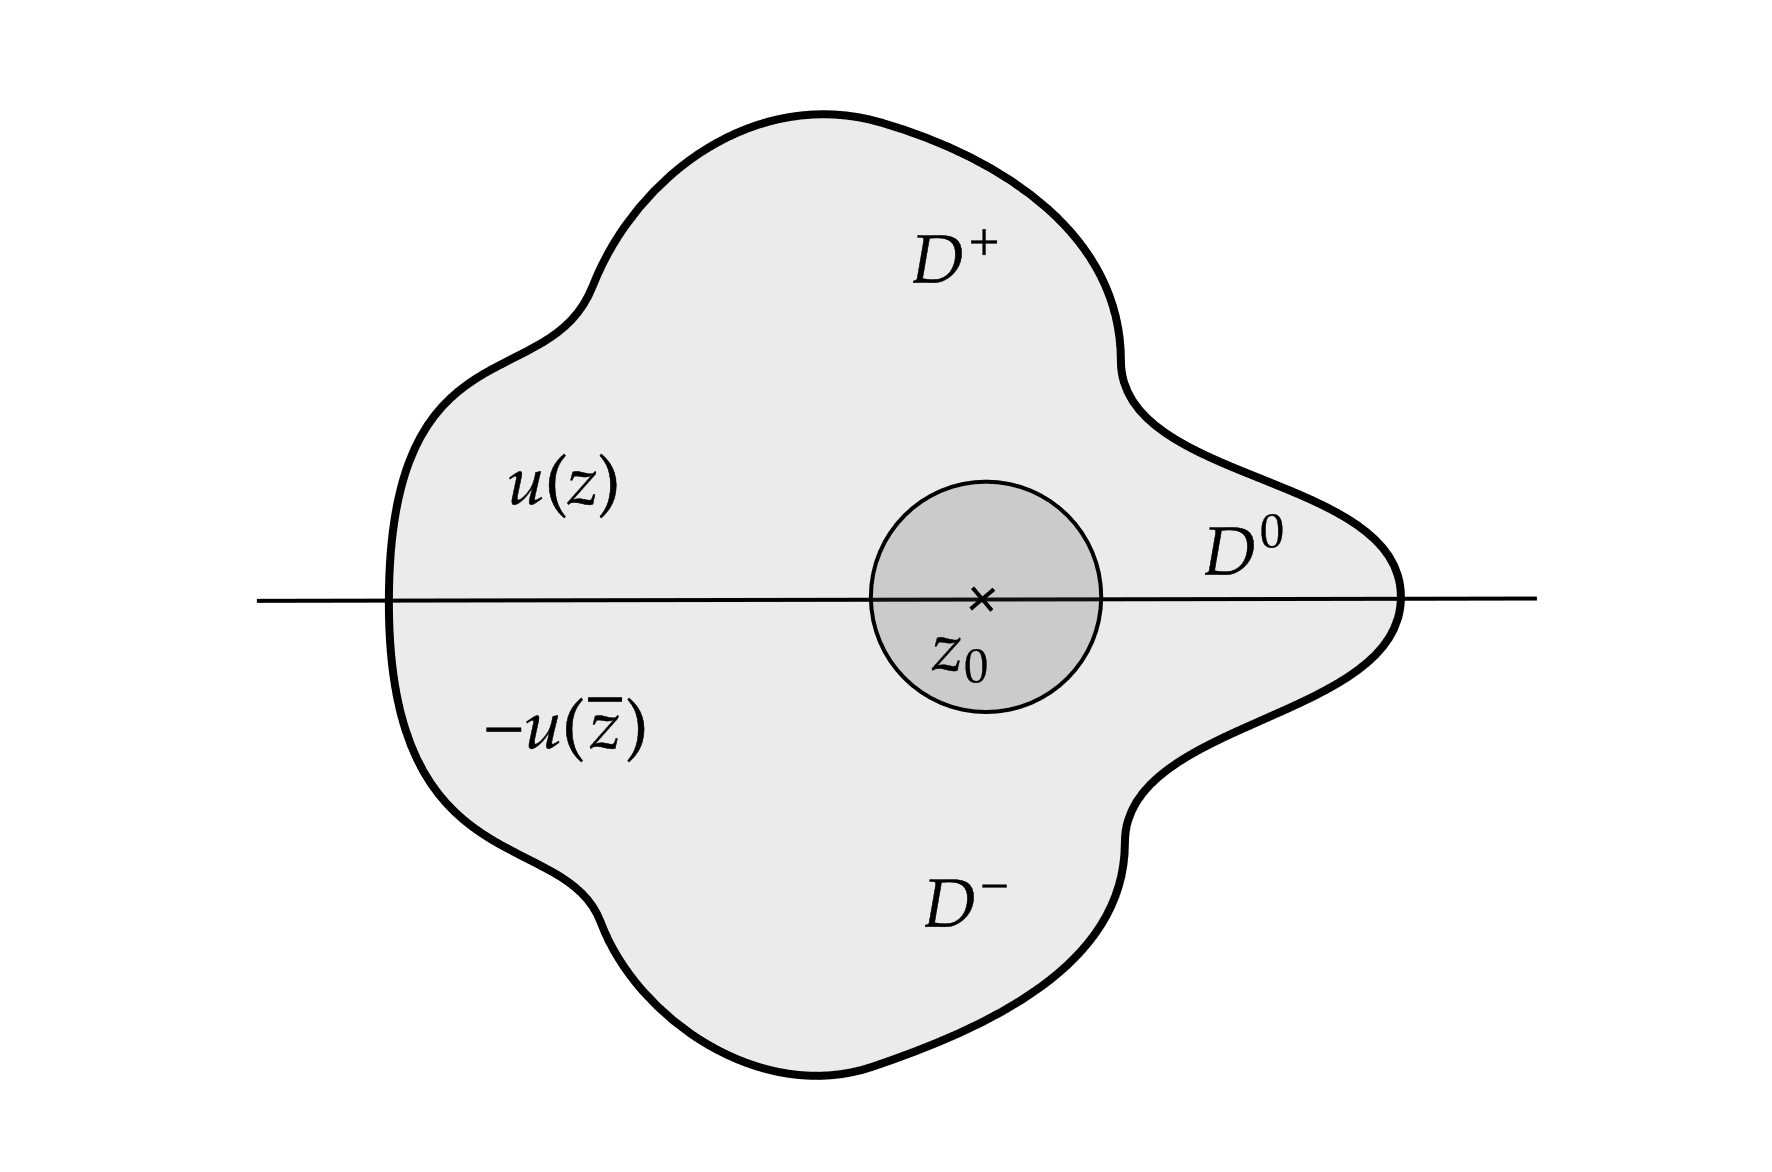
\includegraphics[width=\textwidth]{schwarz_harm.png}
   \end{center}
   \end{figure}
\end{frame}

\begin{frame}{Schwarzov princip zrcaljenja za holomorfne funkcije}
    \begin{exampleblock}{Izrek (Schwarzov princip zrcaljenja za holomorfne funckije)}
        Naj bo $D \subseteq \mathbb{C}$ območje, simetrično glede na realno os. 
        Označimo $D^{+} = \{z \in D~|~\text{Im}[z] > 0\},~D^{-} = \{z \in D~|~\text{Im}[z] < 0\}$ in $D^{0} = \{z \in D~|~\text{Im}[z] = 0\}$.
        Naj bo $f$ zvezna funkcija, definirana na $D^{+} \cup D^0$. Naj bo $f$ na $D^{+}$ holomorfna in naj $f$ na $D^0$ zavzame realne vrednosti.
        Potem je funkcija $F$, definirana s predpisom
        $$
        F(z) = 
        \begin{cases}
            f(z)~,~~&z \in D^{+} \cup D^0\\
            \overbar{f(\overbar{z})}~,~~&z \in D^{-} \cup D^0
        \end{cases}~,
        $$
        na območju $D$ holomorfna.
    \end{exampleblock}
\end{frame}


% -------------------------------------------------------------------
%---------------------------------------------------------
\end{document}
